\documentclass[a4paper, 11pt]{report}

\usepackage[utf8]{inputenc} % Définit l'encodage du document
\usepackage[T1]{fontenc} % Définit l'encodage de la fonte
\usepackage[francais]{babel} % Spécifie que le document est en français
\usepackage{graphicx}
\graphicspath{{.}}

\usepackage{lipsum}

\begin{document}
        \title{BE 3 - Extraction de connaissances}
        \author{Jordan \bsc{Abderrachid}\\ Thomas \bsc{Perrot}\\ Louis \bsc{Zawadski}}

        \maketitle


        \section{Exercice 1}
        \begin{table}[h!]
            \centering
        	\begin{tabular}{|c|c|c|c|c|c|}
        		\hline
        		Cluster & Outlook & Température & Humidity & Windy & Play \\
        		\hline
        		Cluster0 : & overcast & 72.0 & 90.0 & TRUE & yes \\
        		\hline
        		Cluster1 : & sunny & 85.0 & 85.0 & FALSE & no \\
        		\hline
        	\end{tabular}
        \end{table}
        \section{Exercice II}
        On applique l'algorithme \emph{SimpleKMeans} à la base de données \emph{weather.arff}. On obtient les résultats présentés dans le tableau ci-dessous.
        
        \begin{table}[h!]
        \centering
        \begin{tabular}{| l | l | l | l | l | l |}
        \hline
        Cluster & Outlook & Temperature & Humidity & Windy & Play \\
        \hline
        Cluster 0 & sunny & 75.9 & 84.1 & FALSE & yes \\
        \hline
        Cluster 1 & overcast & 69.4 & 77.2 & TRUE & yes \\
        \hline

        \end{tabular}
        \caption{Centroïdes calculés par l'algorithme \emph{SimpleKMeans} avec 2 clusters}
        \label{tab:exo_2}
        \end{table}
        
        \section{Exercice III}
        On peut remarquer que les centroïdes des clusters sont beaucoup plus proches dans le cas de \emph{SimpleKMeans}. Par ailleurs, l'algorithme Fartherst-First génère un cluster correspondant à Play=no et un autre à Play=yes. On peut donc en déduire que l'algorithme qui maximise le plus la dispersion inter-cluster est l'algorithme Farthest-First.
        
        \section{Exercice VI}
        On change le paramètre seed de l'algorithme \emph{SimpleKMeans}. On remarque que les clusters sont initialisés avec play=yes pour l'un et play=no pour l'autre.
        \begin{table}[h!]
        \centering
        \begin{tabular}{| l | l | l | l | l | l |}
        \hline
        Cluster & Outlook & Temperature & Humidity & Windy & Play \\
        \hline
        Cluster 0 & sunny & 75 & 84.1 & FALSE & yes \\
        \hline
        Cluster 1 & sunny & 71 & 77.2 & TRUE & no \\
        \hline

        \end{tabular}
        \caption{Centroïdes calculés par l'algorithme \emph{SimpleKMeans} avec un seed différent}
        \label{tab:exo_6}
        \end{table}
        
        \section{Exercice VII}
        On visualise les résultats obtenus par la simulation précédente. On remarque que les combinaisons de valeurs suivantes appartiennent au cluster 0 :
        \begin{table}[h!]
        \centering
        \begin{tabular}{| c | c |}
         \hline
         Outlook & Windy \\
         \hline
         sunny & false \\
         overcast & false \\
         rainy & false \\
         \hline
        
        \end{tabular}
        \caption{Couples Outlook-Windy appartenant au cluster 0}
        \label{tab:exo7_1}
        \end{table}
        
        Les couples suivants appartiennent au cluster 1 : 
        \begin{table}[h!]
        \centering
        \begin{tabular}{| c | c |}
         \hline
         Outlook & Windy \\
         \hline
         sunny & true \\
         rainy & true \\
         \hline
        
        \end{tabular}
        \caption{Couples Outlook-Windy appartenant au cluster 1}
        \label{tab:exo7_2}
        \end{table}
        
        \section{Exercice VIII}
        On compare les résultats obtenus avec \emph{Farthest-First} et \emph{SimpleKMeans}. On peut remarquer que les couples de valeurs outlook-windy suivantes ont des clusters différents selon la classification : 
        \begin{table}[h!]
        \centering
        \begin{tabular}{| c | c |}
         \hline
         Outlook & Windy \\
         \hline
         sunny & false \\
         overcast & true \\
         rainy & true\\
         \hline
        
        \end{tabular}
        \caption{Couples Outlook-Windy ayant des clusters différents}
        \label{tab:exo8}
        \end{table}
        
        \section{Exercice IX}
        On affiche côte-à-côte les graphiques représentant l'appartenance au cluster et l'attribut play pour les couples de valeurs Outlook-Windy.
        On remarque des différences pour les couples de valeur suivants :
        \begin{table}[h!]
        \centering
        \begin{tabular}{| c | c |}
         \hline
         Outlook & Windy \\
         \hline
         sunny & false \\
         sunny & true \\
         \hline
        
        \end{tabular}
        \caption{Couples Outlook-Windy ayant des valeurs de play et des clusters différents}
        \label{tab:exo9}
        \end{table}
        
        
        \section{Exercice XVI}
        On effectue l'algorithme EM pour différentes valeurs de seed. On obtient les mêmes résultats pour toutes les valeurs de seed de 1 à 1000, à savoir celle présentée dans le tableau ci-dessous : 
        \begin{table}[h!]
        \centering
        \begin{tabular}{| c | c | c | c | c |}
        \hline
         Algo & Seed & Taux d'erreur & Faux négatifs & Faux positifs  \\
         \hline
         EM & x & 35\% & 2 & 3 \\
         \hline
         
        \end{tabular}
        \caption{Résultats de l'algorithme EM}
        \label{tab:exo16}
        \end{table}
        
        \section{Exercice XVII}
        On peut relever les valeurs les plus probables dans les clusters générés par la méthode EM :
        \begin{table}[h!]
        \centering
        \begin{tabular}{| l | l | l | l | l | l |}
        \hline
        Cluster & Outlook & Temperature & Humidity & Windy & Play \\
        \hline
        Cluster 0 & rainy & 70.2 & 80.7 & TRUE & yes \\
        \hline
        Cluster 1 & overcast & 82.2 & 84.0 & FALSE & no \\
        \hline

        \end{tabular}
        \caption{Valeurs les plus probables dans les clusters EM}
        \label{tab:exo_6}
        \end{table}
        
        \section{Exercice XVIII}
        On teste l'algorithme Cobweb avec différentes valeurs pour le \emph{CutOff}. On remarque que l'on obtient 2 clusters pour un \emph{CutOff} de 0,24. On obtient le résultat suivant : 
        
        \begin{table}[h!]
        \centering
        \begin{tabular}{| c | c | c | c | c |}
        \hline
         Algo & CutOff & Taux d'erreur & Faux négatifs & Faux positifs  \\
         \hline
         Cobweb & 0.24 & 35\% & 3 & 2 \\
         \hline
         
         
        \end{tabular}
        \caption{Résultats de l'algorithme Cobweb}
        \label{tab:exo18}
        \end{table}
        
        \section{Exercice XX (Bonus)}
        On applique les algorithmes \emph{Cobweb} et \emph{EM} à la base de données titanic.arff. On obtient les résultats suivants :
        \begin{table}[h!]
        \centering
        \begin{tabular}{| c | c | c | c | c |}
        \hline
         Algo & CutOff/Seed & Taux d'erreur & Faux négatifs & Faux positifs  \\
         \hline
         Cobweb & 0.175 & 22\% & 367 & 126 \\
         \hline
         EM & 10 & 46\% & 212 & 817 \\
         \hline
         
        \end{tabular}
        \caption{Comparaison Cobweb et EM sur la base titanic}
        \label{tab:exo20}
        \end{table}
        
        On peut déduire de ces résultats que l'algorithme Cobweb sont meilleurs que celui de l'algorithme EM.
        
        \section{Exercice XXIV}
        On applique K-means ++ à la base de données bank-data. On observerve les meilleurs résultats pour $seed = 10$. Pour cette valeur de seed on obtient les résultats suivants sur les 60 instances de test :
        
        \begin{table}[h!]
        \centering
        \begin{tabular}{| c | c | c | c | c |}
        \hline
         Algo & Seed & Taux d'erreur & Faux négatifs & Faux positifs  \\
         \hline
         K-means++ & 10 & 16\% & 4 & 6 \\
         \hline
        \end{tabular}
        \caption{Application de k-means ++}
        \label{tab:exo24}
        \end{table}
        
        \section{Exercice XXV}
        On applique la méthode de classification J48 à l'ensemble de test en demandant de déterminer le cluster. On parvient à classer correctement toutes les instances grâce aux règles suivantes : 
        \begin{table}[h!]
        \centering
        \begin{tabular}{l l l l}
        Si pep=YES & & & \\
         // & Si sex = FEMALE & & \\
         // & // & Si car = NO & alors cluster NO \\
         // & // & Si car = YES & alors cluster YES \\
         // & Si sex = MALE & & alors cluster YES \\
        Si pep = NO & & & \\
         // & Si car = NO & & alors cluster NO \\
         // & Si car = YES & & \\
         // & // & Si sex = FEMALE & alors cluster NO \\
         // & // & Si sex = MALE & alors cluster YES\\
        \end{tabular}
        \caption{Règles de classification de l'ensemble de test clusterisé}
        \label{tab:exo25}
        \end{table}
        
        \section{Exercice XXVI}
        On applique K-means ++ à l'ensemble des instances de la base de données bank-data.
        On obtient le meilleur résultat pour un seed de 52. On obtient alors les valeurs suivantes :
        \begin{table}[h!]
        \centering
        \begin{tabular}{| c | c | c | c | c |}
        \hline
         Algo & Seed & Taux d'erreur & Faux négatifs & Faux positifs  \\
         \hline
         K-means++ & 52 & 42\% & 145 & 108 \\
         \hline
        \end{tabular}
        \caption{Application de k-means ++}
        \label{tab:exo26}
        \end{table}
        
        On remarque que cette méthode de clustering n'est pas très efficace.
        
        
        \section{Exercice XXVII}
        On applique la méthode de classification J48 à la base de données ainsi clusterisée. On obtient les règles suivantes :
        \begin{figure}[h!]
        \centering
        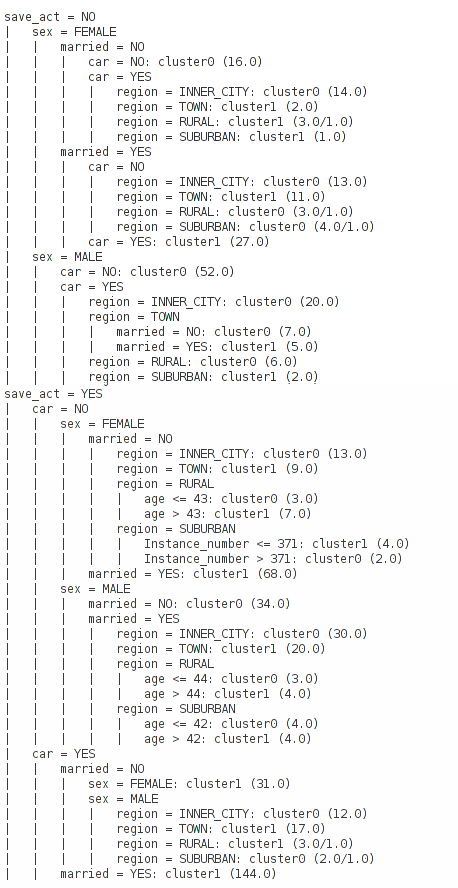
\includegraphics[scale=0.4]{regles27}
        \caption{Règles de classification}
        \label{fig:exo27}
        \end{figure}

        
        
\end{document}
